\section{Slip Ring Connector}\label{sec:ring_connector}
The board with the LEDs will be rotating, making the communication to this board a problem.
Existing solutions called slip rings exist, but the ones in the price range of this project is rated for 250 rpm, which will be too slow for this project.
So a custom solution will be devised to combat this.

To make communication between the rotating board and the stationary FPGA, a slip ring connector is made.
This was made as two Eagle components so the sizes are identical.
In figure \ref{fig:slip_ring_eagle} is the slip ring shown.
The bottom layer contains rings where the signal is sent to.
The top layer has pads directly over the rings and by having a wire that touches the ring, the connection can be made.
The outer layers are used for signals.
This allows for multiple wires to have contact with the ring.
The power supply is stabilized with a $220 \mu F$ capacitor.
This is done to stabilize the power signal and to make sure the LED drivers does not disconnect if the wire loses contact for a moment.
The duration of this disconnect is hard to determine, so the a large capacitor is chosen to maximize the lifespan in case of a disconnect.

The LED driver requires a signal for power, ground, input signal, a clock and a latch.
Having multiple drivers does not increase the number of wires.

\begin{figure}[h]
 \centering
 \begin{subfigure}{0.4\linewidth}
  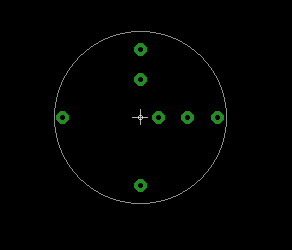
\includegraphics[width=\linewidth]{img/slip_ring_top}
 \caption{Top layer.}
 \label{fig:slip_ring_top}
 \end{subfigure}
 \begin{subfigure}{0.4\linewidth}
  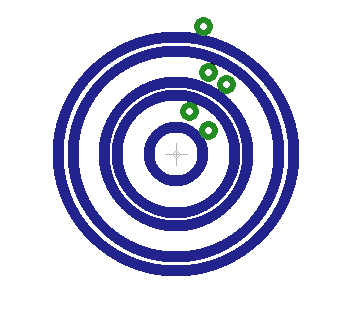
\includegraphics[width=\linewidth]{img/slip_ring_bot}
 \caption{Bottom layer.}
 \label{fig:slip_ring_bot}
 \end{subfigure}
 \caption{Slip ring component made in Eagle.}
 \label{fig:slip_ring_eagle}
\end{figure}

% \begin{figure}[h]
%     \centering
%     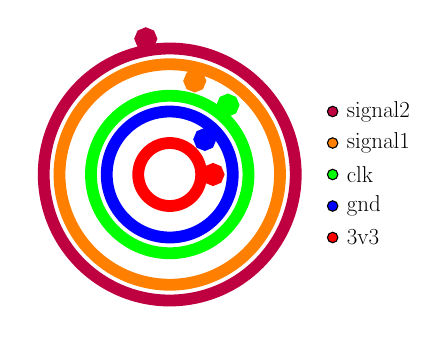
\begin{tikzpicture}[scale = 0.4, every node/.style={scale=0.4}]
      \def\ringwidth{0.15}
      \def\offA{0.3}	
      \def\offB{-0.5}

      %rings
      \node[draw, circle, line width=\ringwidth cm, rotate=0  ,  color = red    , minimum width=2.0cm, name=3v3    ] at (0,0) {}; 
      \node[draw, circle, line width=\ringwidth cm, rotate=45 ,  color = blue   , minimum width=4.0cm, name=gnd    ] at (0,0) {}; 
      \node[draw, circle, line width=\ringwidth cm, rotate=50 ,  color = green  , minimum width=5.0cm, name=clk    ] at (0,0) {}; 
      \node[draw, circle, line width=\ringwidth cm, rotate=75 ,  color = orange , minimum width=7.0cm, name=signal1] at (0,0) {}; 
      \node[draw, circle, line width=\ringwidth cm, rotate=100,  color = purple , minimum width=8.0cm, name=signal2] at (0,0) {}; 
      
      %pads
      \draw[red    , line width=\ringwidth cm, rotate=0  ]     (3v3.0) -- ++(\offA,0) node[draw, circle, fill= red    , minimum width=0.25cm] {};
      \draw[blue   , line width=\ringwidth cm, rotate=45 ]     (gnd.0) -- ++(\offB,0) node[draw, circle, fill= blue   , minimum width=0.25cm] {};
      \draw[green  , line width=\ringwidth cm, rotate=50 ]     (clk.0) -- ++(\offA,0) node[draw, circle, fill= green  , minimum width=0.25cm] {};
      \draw[orange , line width=\ringwidth cm, rotate=75 ] (signal1.0) -- ++(\offB,0) node[draw, circle, fill= orange , minimum width=0.25cm] {};
      \draw[purple , line width=\ringwidth cm, rotate=100] (signal2.0) -- ++(\offA,0) node[draw, circle, fill= purple , minimum width=0.25cm] {};
      
      %legend
      \draw 
      (0,0) ++( 5  ,-2) node[draw, circle, right, fill = red   ] {} ++(0.5,0) node[right] {\huge 3v3    }
	    ++(-0.5, 1) node[draw, circle, right, fill = blue  ] {} ++(0.5,0) node[right] {\huge gnd    }
	    ++(-0.5, 1) node[draw, circle, right, fill = green ] {} ++(0.5,0) node[right] {\huge clk    }
	    ++(-0.5, 1) node[draw, circle, right, fill = orange] {} ++(0.5,0) node[right] {\huge signal1}
	    ++(-0.5, 1) node[draw, circle, right, fill = purple] {} ++(0.5,0) node[right] {\huge signal2}
      ;
\end{tikzpicture}
%     \caption{Sketch of the schematic side of the slip ring.}
%     \label{fig:slip_ring_tikz}
% \end{figure}